\chapter*{Diagram}

\tikzset{tight/.style={
    inner sep=0pt, 
    outer sep=0pt,
    node distance=1em
}}

\def\nouncontent{%
    \begin{tikzpicture}[every node/.style={tight}]
        \node (rect1)  at (0,0) {\rect[color=gray, width=4em, height=1.8em, label={gender}]};%
        \node (rect2) [right=of rect1] {\rect[color=gray, width=4em, height=1.8em, label={number}]};%
        \node (rect3) [right=of rect2] {\rect[color=gray, width=4em, height=1.8em, label={case}]};%

        \node (pill1) [below=of rect1] {\pill[color=gray, scale=1.2, label=\hyperref[table:artdef]{art.def.}]};%
        \node (pill2) [right=of pill1] {\pill[color=gray, scale=1.2, label={pron.3.per}]};%
        \node (pill3) [right=of pill2] {\pill[color=gray, scale=1.2, label={adj.str.}]};%
        \draw[-, shorten >=0, shorten <=0] (pill1) -- (pill2) node[midway, above] {};%
        \draw[-, shorten >=0, shorten <=0] (pill2) -- (pill3) node[midway, above] {};%

        \node (pill4) [below=of pill1] {\pill[color=gray, scale=1.2, label={art.indef.}]};%
        \node (pill5) [right=of pill4] {\pill[color=gray, scale=1.2, label={pron.3.pos.}]};%
        \node (pill6) [right=of pill5] {\pill[color=gray, scale=1.2, label={adj.wk.}]};%
        \draw[-, shorten >=0, shorten <=0] (pill4) -- (pill5) node[midway, above] {};%
        \draw[-, shorten >=0, shorten <=0] (pill5) -- (pill6) node[midway, above] {};%
    \end{tikzpicture}
}

\def\verbcontent{%
    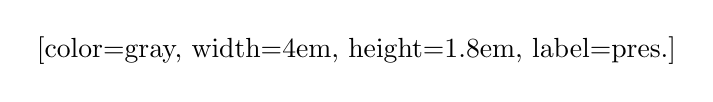
\begin{tikzpicture}[node distance=1em]
        \node (rect1)  at (0,0) {\rect[color=gray, width=4em, height=1.8em, label={pres.}]};%
    \end{tikzpicture}
}

\def\prepcontent{%
    \begin{tikzpicture}[node distance=1em]
    \end{tikzpicture}
}

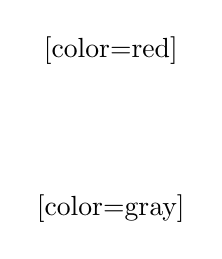
\begin{tikzpicture}[]
    % \node(cir1) at (0, 0){\cir[color=yellow, border=1, scale=2]};
    \node(flower1) at (0, 0){\flower[color=gray]};
    \node(flower1) at (0, 2){\square[color=red]};

    % \node (card1) at (0, 0) {\card[width=17em,height=10em,label=\hyperref[chap:noun]{noun}]{\nouncontent}};
    % \node (card2) [below=of card1] {\card[width=17em,height=8em,label=\hyperref[chap:noun]{verb}]{\verbcontent}};
    % \node (card3) [right=of card2] {\card[width=17em,height=8em,label=\hyperref[chap:noun]{prep}]{\prepcontent}};
    % \node (card4) [below=of card2] {\card[width=17em,height=8em,label=\hyperref[chap:noun]{syntax}]{\prepcontent}};

    % \draw[-latex, shorten >=0, shorten <=0] (card2) -- (card1) node[midway, above] {case};
    % \draw[-latex, shorten >=0, shorten <=0] (card3) -- (card1) node[midway, above] {case};
\end{tikzpicture}